\section{CIC Filter}
The CIC filter is implemented by using Xilinx IP core. Filters' purpose in the design is to provide decimation, to reduce number of samples by 10. It means that the sampling rate is 100 MHz from the main clock and after the processing by the filter the sampling will be 10 MHz. The ready signal for all blocks is working in a chain. It means when a block is finish and delivers the result to the next block with a ready signal as control signal. This core has latency on 15.

\section{Cordic}
This block is implemented by using Xilinx IP core. The Cordic get two inputs respectively I and Q from CIC Filters. The Cordic performs Vector Translation on the inputs to transform rectangular to polar which is amplitude and phase. In this design the phase output is only useful, because the amplitude only concerning AM modulation. This core has latency on 20. The Cordic phase output can be seen in figure \ref{fig:cordic}. In the figure we can see some transitions from positive to negative and vice versa. The reason is that the Cordic only can provides output from $-\pi$ to $\pi$. It will show later, that these transitions will cause problems.

\begin{figure}[h]
 \centering
 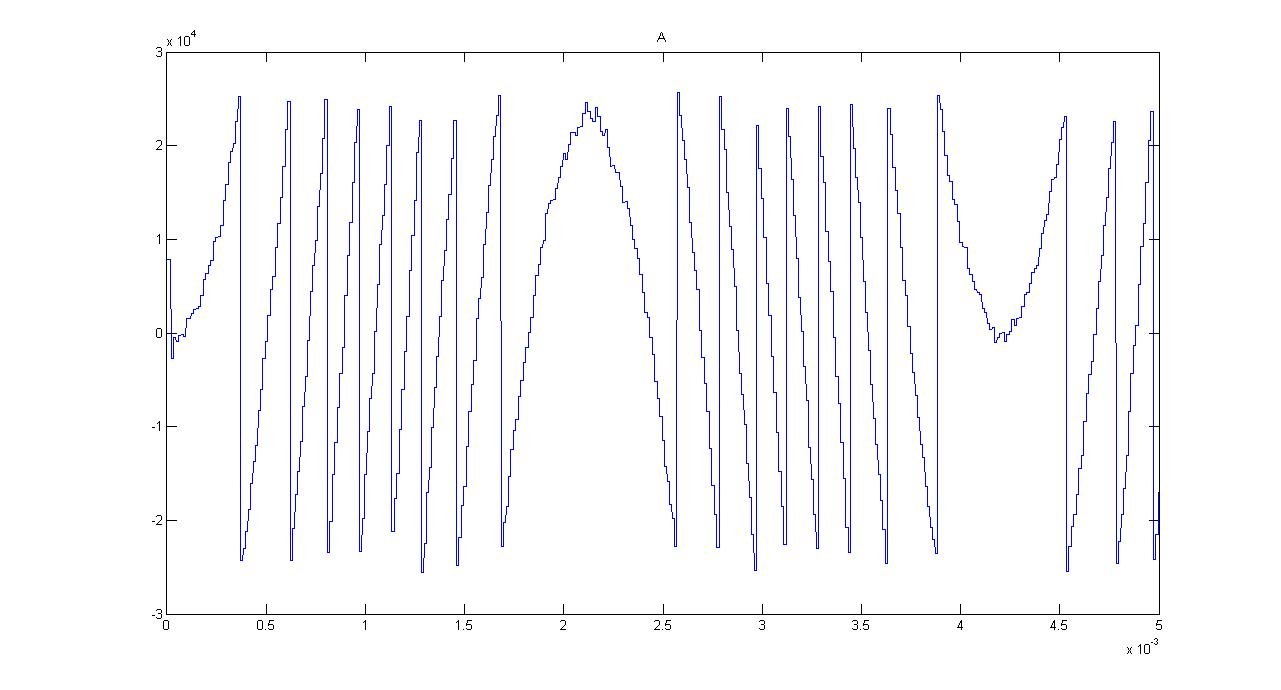
\includegraphics[scale=0.2]{images/cordic.jpg}
 \caption{Phase output of the Coridc}
 \label{fig:cordic}
\end{figure}

\section{Shiftregister}
The differential filter requires previous sample, x(n), x(n-2),x(n-4),x(n-6). The shiftregister will shift all the samples, when a new sample is read. The process is illustrated in figure \ref{fig:shift}.

\begin{figure}[h]
 \centering
 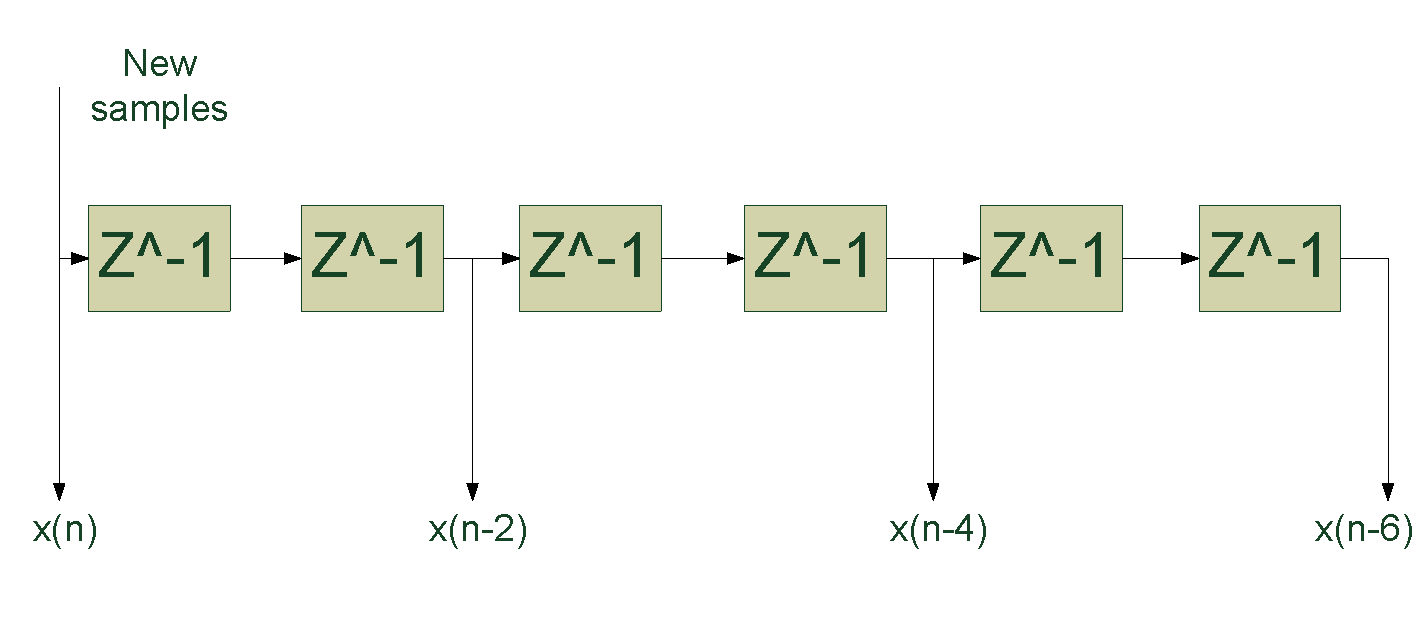
\includegraphics[scale=0.4]{images/shift.pdf}
 \caption{Shiftregiser process}
 \label{fig:shift}
\end{figure}

\section{Click Remover}
The purpose of this block is to avoid clicks in the final output. The output when the click remover is disabled can be seen in figure \ref{fig:clicks}. This part of the design was one the more difficult to fine-tune the click remover so it removes all clicks. These clicks occur when the differential filter uses the sequence of samples which contains a transition from positive to negative or versa visa. First the clicks will be detected by comparing $x(n) - x(n-6) > \pi$ or $x(n) - x(n-6) < -\pi$. If a click is detected, the algorithm will add two $\pi$ to the four samples, if the samples are less than zero. After this operation the sample interval will be continuous(It is continuous when this specific transition isn't present). The illustration can be seen in figure \ref{fig:remove}.

\begin{figure}[h]
 \centering
 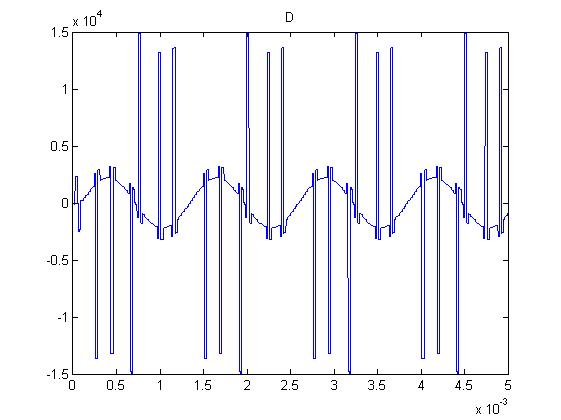
\includegraphics[scale=0.4]{images/clicks.jpg}
 \caption{The final output with clicks}
 \label{fig:clicks}
\end{figure}

\begin{figure}[h]
 \centering
 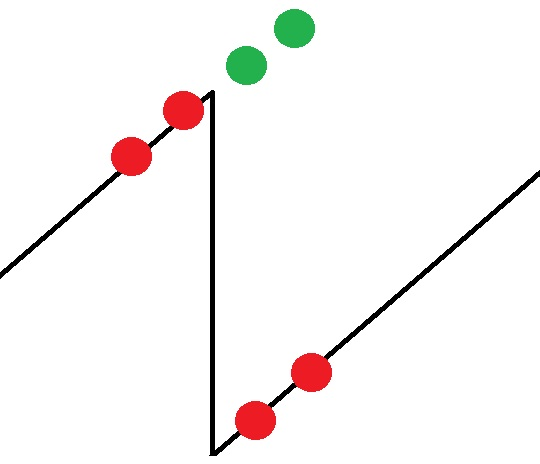
\includegraphics[scale=0.4]{images/remove.jpg}
 \caption{The red points are the original samples, it makes this discontinuity. The green points are the result of the click remover.}
 \label{fig:remove}
\end{figure}

\section{Differential filter}
This differentiator is the most usable for this design. It has high frequency attenuation and a reasonably linear operation up to $0,17f_s Hz$. The differentiator is defined by

\begin{align}
	y_{diff} = \frac{-x(n)}{16} + x(n-2) - x(n-4) + \frac{x(n-6)}{16}
\end{align}

The output is the final result of the demodulation for 500 $\mu s$, it is present in figure \ref{fig:pure}.

\begin{figure}[h]
 \centering
 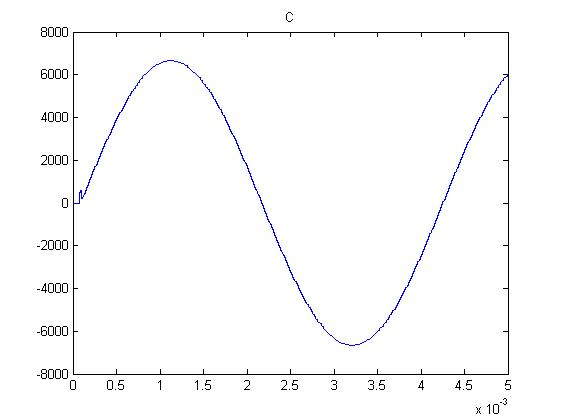
\includegraphics[scale=0.4]{images/ypure.jpg}
 \caption{Output of the demodulation}
 \label{fig:pure}
\end{figure}

It can be noticed that there is some setting time in start of the process.